There are a large number of tools that can be used to read in \castro\
or \boxlib\ data and make plots.  Here we give a brief overview of some
of the tools as well as some examples.

\section{Controlling What's in the PlotFile}

There are a few options that can be set at runtime to control what
variables appear in the plotfile.

{\bf amr.plot\_vars} = \\

\noindent and  \\

\noindent {\bf amr.derive\_plot\_vars} = \\

\noindent are used to control which variables are included in the plotfiles.  The default for {\bf amr.plot\_vars}
is all of the state variables.  The default for {\bf amr.derive\_plot\_vars} is none of
the derived variables.  So if you include neither of these lines then the plotfile
will contain all of the state variables and none of the derived variables. \\

\noindent If you want all of the state variables plus entropy and pressure, for example, then set \\

\noindent {\bf amr.derive\_plot\_vars} = entropy pressure \\

\noindent If you just want density and pressure, for example, then set \\

\noindent {\bf amr.plot\_vars} =  density \\

\noindent {\bf amr.derive\_plot\_vars} = pressure \\



\section{amrvis}
Our favorite visualization tool is amrvis. We heartily encourage you
to build the amrvis2d and amrvis3d executables, and to try using them
to visualize your data. A very useful feature is View/Dataset, which
allows you to actually view the numbers -- this can be handy for
debugging. You can modify how many levels of data you want to see,
whether you want to see the grid boxes or not, what palette you use,
etc.

If you like to have amrvis display a certain variable, at a certain
scale, when you first bring up each plotfile (you can always change it
once the amrvis window is open), you can modify the amrvis.defaults
file in your directory to have amrvis default to these settings every
time you run it. The directories CoreCollapse, HSE\_test, Sod and
Sedov have amrvis.defaults files in them. If you are working in a new
run directory, simply copy one of these and modify it.


\section{VisIt}
VisIt is also a great visualization tool, and it directly handles our
plotfile format (which it calls Boxlib).  For more information check
out visit.llnl.gov.

[Useful tip:] To use the Boxlib3D plugin, select it from File
$\rightarrow$ Open file $\rightarrow$ Open file as type Boxlib, and
then the key is to read the Header file, plt00000/Header, for example,
rather than telling to to read plt00000.

\section{\yt}
\yt\ is a free and open-source software that provides data analysis and
publication-level visualization tools for astrophysical simulation
results such as those CASTRO produces. As \yt\ is script-based, it's not
as easy to use as VisIt, and certainly not as easy as amrvis, but the
images can be worth it! Here we do not flesh out \yt, but give an
overview intended to get a person started. Full documentation and
explanations from which this section was adapted can be found at
http://yt-project.org/doc/index.html.

\yt\ can be installed by the following commands:

\$ wget http://hg.yt-project.org/yt/raw/stable/doc/install\_script.sh

\$ bash install\_script.sh

This installs \yt\ in your current directory. To update \yt in the
future, simply do

\$ yt update

in your ``yt-hg'' folder.

\subsection{Castro-Specific Data}

\yt\ was originally created for simple analysis and visualization of
data from the Enzo code. Since, it has grown to include support for a
variety of codes, including Castro. However, \yt will still sometimes
make assumptions, especially about data field names, that favor Enzo
and cause errors with Castro data. These problems can usually be
avoided by taking care to specify the data fields desired in
visualization. For example, Enzo's density field is called
``Density,'' and is the default for many plotting mechanisms when the
user does not specify the field. However, Castro does not have a field
called ``Density''; instead, the density field is called ``density.''
If a user does not specify a field while plotting with Castro data,
chances are that \yt\ will try (and fail) to find ``Density'' and return
an error. As you will see in the examples, however, there is a way to
create your own fields from existing ones. You can use these derived
fields as you would use any other field.

There are also a few imperatives when it comes to reading in your
Castro simulation data and associated information. First and foremost
is that the inputs file for the simulation {\bf must} exist in the
same directory as where the plotfile directory is located, and it {\bf
  must} be named ``{\bf inputs}.'' \yt\ reads information from the
inputs file such as the number of levels in the simulation run, the
number of cells, the domain dimensions, and the simulation time. \yt\
will also optionally parse the probin file for pertinent information
if it is similarly included with the name ``{\bf probin}'' in the same
directory as the plotfile of interest. When specifying a plotfile as
the data source for plots, you may simply call it by its directory
name, rather than using the Header file as in VisIt. As a final
caveat, the existence of the job\_info file within the plotfile
directory is what currently distinguishes Castro data from MAESTRO
data in \yt; unless you like surprises, we suggest you ensure your
plotfile has one.

\subsection{Interacting with \yt: Command Line and Scripting}

\yt is written completely in python (if you don't have python, \yt\ will
install it for you) and there are a number of different ways to
interact with it, including a web-based gui. Here we will cover
command-line \yt\ and scripts/the python interactive prompt, but other
methods are outlined on the \yt\ webpage at
http://yt-project.org/doc/interacting/index.html.

The first step in starting up \yt\ is to activate the \yt\ environment:

\$ source \$YT\_DEST/bin/activate

From the command line you can create simple plots, perform simple
volume renderings, print the statistics of a field for your data set,
and do a few other things. Try {\$ \tt yt} to see a list of commands,
and {\$ \tt yt {\footnotesize$<$}command{\footnotesize$>$} -{}-help}
to see the details of a command. The command line is the easiest way
to get quick, preliminary plots -- but the simplicity comes at a
price, as \yt\ will make certain assumptions for you. We could plot a
projection of density along the x-axis for the plotfile (\yt\ calls it a
parameter file) plt\_def\_00020 by doing the following:

\$ yt plot -p -a 0 -f density plt\_def\_00020

Or a temperature-based volume rendering with 14 contours:

\$ yt render -f Temp -{}-contours 14 plt\_def\_00020

Any plots created from the command line will be saved into a
subdirectory called ``frames.'' The command line is nice for fast
visualization without immersing yourself too much in the data, but
usually you'll want to specify and control more details about your
plots. This can be done either through scripts or the python
interactive prompt. You can combine the two by running scripts within
the interactive prompt by the command

{\scriptsize$>>>$} execfile(`script.py')

which will leave you in the interactive prompt, allowing you to
explore the data objects you've created in your script and debug
errors you may encounter. While in the \yt\ environment, you can access
the interactive prompt by {\$ \it python} or the shortcut

\$ pyyt

Once you're in the yt environment and in a .py script or the
interactive prompt, there are a couple of points to know about the
general layout of yt scripting. Usually there are five sections to a
yt script:
\begin{enumerate}
\item
\indent Import modules
\item
\indent Load parameter files and saved objects
\item
\indent Define variables
\item
\indent Create and modify data objects, image arrays, plots,
etc. $\rightarrow$ this is the meat of the script
\item
\indent Save images and objects
\end{enumerate}

Note that neither saving nor loading objects is necessary, but can be
useful when the creation of these objects is time-consuming, which is
often the case during identification of clumps or contours.

\subsection{\yt\ Basics}

The first thing you will always want to do is to import \yt:

{{\scriptsize$>>>$}} from yt.mods import *

Under certain circumstances you will be required to import more, as we
will see in some of the examples, but this covers most of it,
including all of the primary functions and data objects provided by
\yt. Next, you'll need \yt\ to access the plotfile you're interested in
analyzing. Remember, you must have the ``inputs'' file in the same
directory:

{\scriptsize$>>>$} ds = load(`plt\_def\_00020')

When this line is executed, it will print out some key parameters from
the simulation. However, in order to access information about all of
the fluid quantities in the simulation, we must use the ``index''
object. (Note that for yt versions earlier than 3.0, this information
was contained in the ``hierarchy'' object; for these versions, replace
pf.index with pf. h in the following examples. The ``hierarchy'' object
was removed in yt-3.0 and its associated functionality for accessing data
was moved directly to the datasets themselves.) It contains the geometry
of the grid zones, their parentage relationships, and the fluid states
within each one. It is easily created:

{\scriptsize$>>>$} ds.index

Upon execution, \yt\ may print out a number of lines saying it's adding
unknown fields to the list of fields. This is because Castro has
different names for fields than what \yt\ expects. We can see what
fields exist through the commands

{\scriptsize$>>>$} print ds.index.field\_list

{\scriptsize$>>>$} print ds.index.derived\_field\_list

There may not be any derived fields for Castro data. We can find out
the number of grids and cells at each level, the simulation time, and
information about the finest resolution cells:

{\scriptsize$>>>$} ds.index.print\_stats()

The dataset itself also stores a number of associated methods; for example,
you can find the value and location of the maximum of a field in the domain:

{\scriptsize$>>>$} value, location = ds.find\_max(`density')

(Note that in yt versions before 3.0, this type of method was primarily
associated with the hierarchy object and was accessed with ds.h.find\_max.)

The list goes on. A full list of methods and attributes associated
with the index object (and most any \yt\ object or function) can be
accessed by the help function:

{\scriptsize$>>>$} help(pf.index)

You can also use {\scriptsize$>>>$} {\it dir()} on an object or
function to find out which names it defines. Don't be shy about
searching the \yt\ documentation for help. Note that creating the
index object in its own line is not always needed before calling
functions like find\_max; \yt\ will construct it automatically if it
does not already exist.

\subsection{Data Containers and Selection}

Sometimes, you'll want to select, analyze, or plot only portions of
your simulation data. To that end, \yt\ includes a way to create data
``containers'' that select data based on geometric bounds or fluid
quantity values. There are many, including rays, cylinders, and clumps
(some in the examples, all described in the documentation), but the
easiest to create is a sphere, centered on the location of the maximum
density cell we found above:

{\scriptsize$>>>$} my\_data\_container = ds.sphere(location, (5.0e4, `km'))

Here, specify that the radius is in units of kilometers using a dimensionful
quantity. When specifying distances in \yt, the default is to use the
simulation-native unit named ``code\_length'', which for Castro is ``cm'', and
if you just put in 5.0e4 instead of (5.0e4, `km'), you will get a 50,000 cm radius.
The pf.index.print\_stats() command lists available units. We can access the data
within the container:

{\scriptsize$>>>$} print my\_data\_container[`density']

{\scriptsize$>>>$} print my\_data\_container.quantities[`Extrema']([`density', `pressure'])

When the creation of objects is time-consuming, it can be convenient
to save objects so they can be used in another session. To save an
object as part of the {\tt .yt} file affiliated with the index:

{\scriptsize$>>>$} pf.index.save\_object(my\_data\_container, `sphere\_to\_analyze\_later')

Once it has been saved, it can be easily loaded later:

{\scriptsize$>>>$} sphere\_to\_analyze = pf.index.load\_object(`sphere\_to\_analyze\_later')

\subsection{Grid Inspection}

\yt\ also allows for detailed grid inspection. The index object
possesses an array of grids, from which we can select and examine
specific ones:

{\scriptsize$>>>$} print pf.index.grids

{\scriptsize$>>>$} my\_grid = pf.index.grids[4]

Each grid is a data object that carries information about its
location, parentage relationships (grids within which it resides, and
grids that reside within it, at least in part), fluid quantities, and
more. Here are some of the commands:

{\scriptsize$>>>$} print my\_grid.Level

{\scriptsize$>>>$} print my\_grid\_ActiveDimensions

{\scriptsize$>>>$} print my\_grid.LeftEdge

{\scriptsize$>>>$} print my\_grid.RightEdge

{\scriptsize$>>>$} print my\_grid.dds

(dds is the size of each cell within the grid).

{\scriptsize$>>>$} print my\_grid.Parent

{\scriptsize$>>>$} print my\_grid.Children[2].LeftEdge

{\scriptsize$>>>$} print my\_grid[`Density']

You can examine which cells within the grid have been refined with the
child\_mask attribute, a representative array set to zero everywhere
there is finer resolution.To find the fraction of your grid that isn't
further refined:

{\scriptsize$>>>$}print my\_grid.child\_mask.sum()/float(my\_grid.ActiveDimensions.prod())

Rather than go into detail about the many possibilities for plotting
in \yt, we'll provide some examples.

\subsection{Example Scripts}

In these examples, we investigate 3-D simulation data of two stars
orbiting in the center of the domain, which is a box of sides
$10^{10}\:cm$.


{\it\# Pressure Contours}
{\setlength{\parskip}{0pt}

from yt.mods import *
}

pf = load(`plt00020')

field = `pressure'

pf.index

{\it\# Most Castro fields have no inherent units, so we add them in,
  in the form of a raw string} 

{\setlength{\parskip}{0pt}

{\it\# with some LaTeX-style formatting.}

pf.field\_info[field].\_units = r`\textbackslash rm\{Ba\}'
}


{\it\# SlicePlot parameters include: parameter file, axis, field, window width (effectively the}
{\setlength{\parskip}{0pt}

{\it\# x and y zoom), and fontsize. We can also create projections with ProjectionPlot().}

p = SlicePlot(pf, `z', field, width=((5.0e9, `cm'), (3.0e9, `cm')),

{\setlength{\parindent}{68pt}fontsize=13)}
}

{\it\# Zlim is the range of the colorbar. In other words, the range of the data we want to display.}
{\setlength{\parskip}{0pt}

{\it\# Names for many colormaps can be found at wiki.scipy.org/Cookbook/Matplotlib/Show\_colormaps.}

p.set\_zlim(field, 2.85e13, 2.95e13)
}

p.set\_cmap(field, `jet')

{\it\# Here we add 5 density contour lines within certain limits on top of the image. We overlay}
{\setlength{\parskip}{0pt}

{\it\# our finest grids with a transparency of 0.2 (lower is more transparent). We add a quiver}

{\it\# plot with arrows every 16 pixels with x\_velocity in the x-direction and y\_velocity in}

{\it\# the y-direction. We also mark the center with an `x' and label one of our stars.}

p.annotate\_contour(`density', clim=(1.05e-4, 1.16e-4), ncont=5, label=False)
}

p.annotate\_grids(alpha=0.2, min\_level=2)

p.annotate\_quiver(`x\_velocity', `y\_velocity', factor=16)

p.annotate\_marker([5.0e9, 5.0e9], marker=`x')

p.annotate\_point([5.95e9, 5.1e9], `Star!')

{\it\# This saves the plot to a file with the given prefix. We can alternatively specify}
{\setlength{\parskip}{0pt}

{\it\# the entire filename.}

p.save(`contours.press\_den\_')
}
%%%%%%%%%%%%%%%%%%%%%%%%%%%%%%%%%
\begin{figure}[h]
\centering
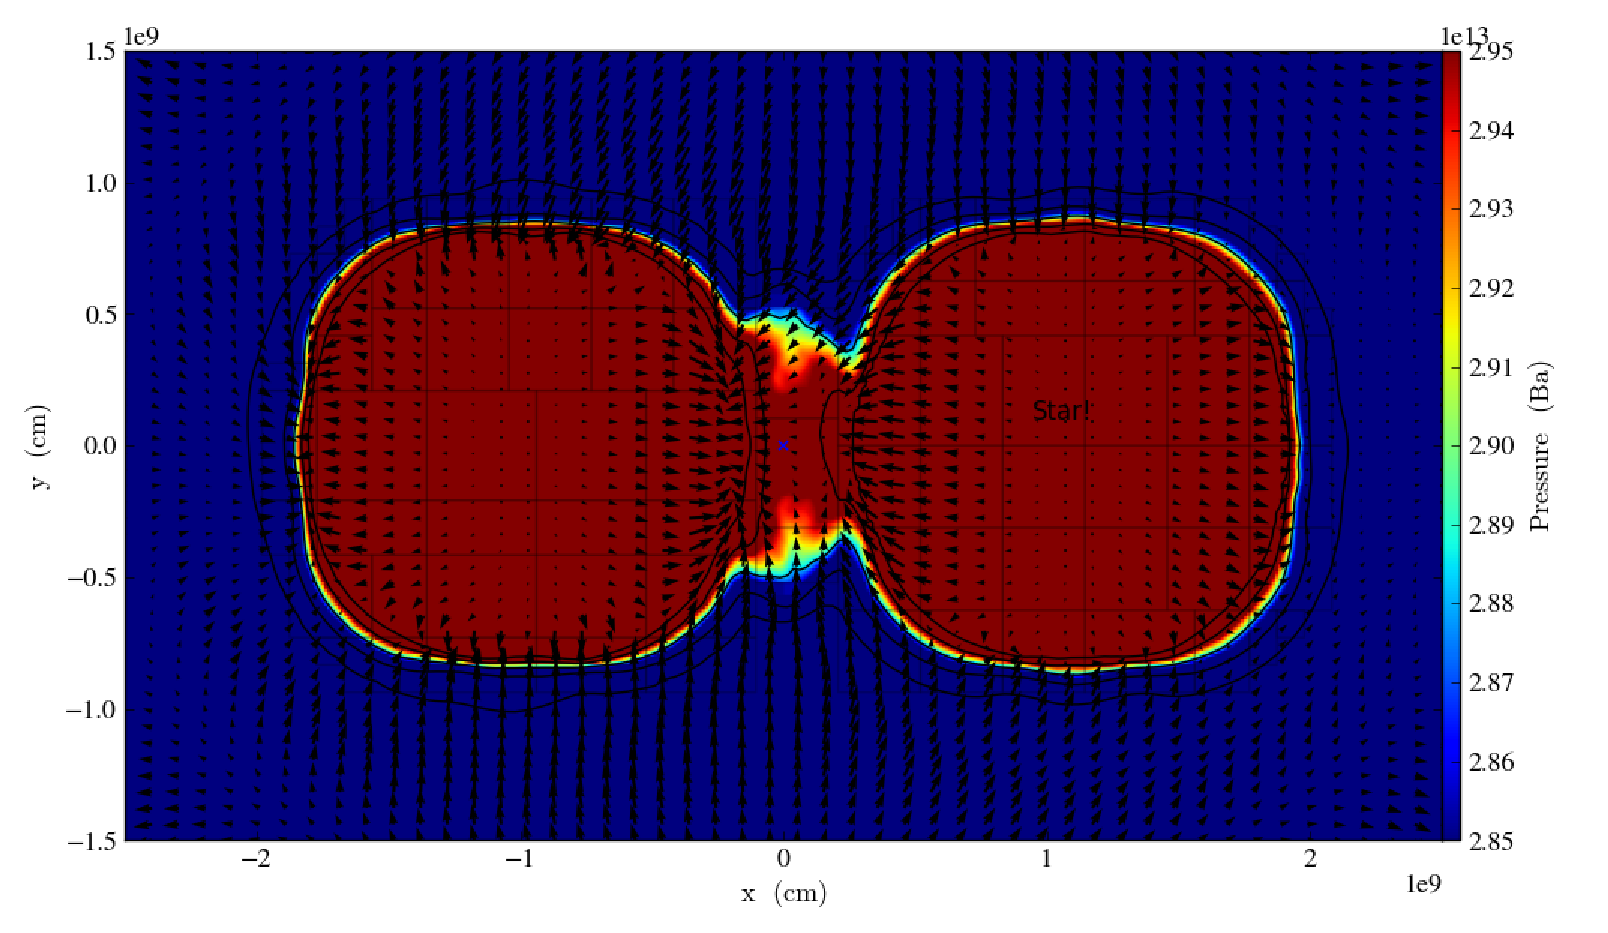
\includegraphics[width=6in]{Slice_z_pressure}
\caption{Pressure slice with annotations}
\end{figure}
%%%%%%%%%%%%%%%%%%%%%%%%%%%%%%%%%

{\it\#------------------------}


{\it\# Volume Rendering}
{\setlength{\parskip}{0pt}

from yt.mods import *
}

pf = load(`plt00020')

field = `pressure'
dd = pf.all\_data()

{\it\# We take the log of the extrema of the pressure field, as well as a couple other interesting}
{\setlength{\parskip}{0pt}

{\it\# value ranges we'd like to visualize.}

h\_mi, h\_ma = dd.quantities[`Extrema'](field)[0]
}

h\_mi, h\_ma = np.log10(h\_mi), np.log10(h\_ma)

s\_mi, s\_ma =  np.log10(2.90e13), np.log10(3.10e13)

pf.index

{\it\# We deal in terms of logarithms here because we have such a large range of values.}
{\setlength{\parskip}{0pt}

{\it\# It can make things easier, but is not necessary.}

pf.field\_info[field].take\_log=True
}

{\it\# This is what we use to visualize volumes. There are a couple of other, more complex}
{\setlength{\parskip}{0pt}

{\it\# ways. We set the range of values we're interested in and the number of bins in the}

{\it\# function. Make sure to have a lot of bins if your data spans many orders of magnitude!}

{\it\# Our raw data ranges from about $10^{13}$ to $10^{22}$.}

tf = ColorTransferFunction((h\_mi-1, h\_ma+1), nbins=1.0e6)
}

{\it\# Here we add several layers to our function, either one at a time or in groups. We}
{\setlength{\parskip}{0pt}

{\it\# specify the value-center and width of the layer. We can manipulate the color by}

{\it\# individually setting the colormaps and ranges to spread them over. We can also}

{\it\# change the transparency, which will usually take some time to get perfect.}

tf.sample\_colormap(np.log10(2.0e21), 0.006, col\_bounds=[h\_mi,h\_ma],
}

{\setlength{\parindent}{96pt}alpha=[27.0], colormap=`RdBu\_r')}

tf.sample\_colormap(np.log10(2.0e19), 0.001, col\_bounds=[h\_mi,h\_ma],

{\setlength{\parindent}{96pt}alpha=[5.5], colormap=`RdBu\_r')}

tf.add\_layers(6, mi=np.log10(2.95e13), ma=s\_ma,

{\setlength{\parindent}{63.5pt}col\_bounds=[s\_mi,s\_ma],}

{\setlength{\parindent}{63.5pt}alpha=19*na.ones(6,dtype=`float64'), colormap=`RdBu\_r')}

tf.sample\_colormap(np.log10(2.95e13), 0.000005, col\_bounds=[s\_mi,s\_ma],

{\setlength{\parindent}{96pt}alpha=[13.0], colormap=`RdBu\_r')}

tf.sample\_colormap(np.log10(2.90e13), 0.000007, col\_bounds=[s\_mi,s\_ma],

{\setlength{\parindent}{96pt}alpha=[11.5], colormap=`RdBu\_r')}

tf.sample\_colormap(np.log10(2.85e13), 0.000008, col\_bounds=[s\_mi,s\_ma],

{\setlength{\parindent}{96pt}alpha=[9.5], colormap=`RdBu\_r')}

{\it\# By default each color channel is only opaque to itself. If  we set grey\_opacity=True,}
{\setlength{\parskip}{0pt}

{\it\# this is no longer the case. This is good to use if we want to obscure the inner}

{\it\# portions of our rendering. Here it only makes a minor change, as we must set our}

{\it\# alpha values for the outer layers higher to see a strong effect.}

tf.grey\_opacity=True
}

{\it\# Volume rendering uses a camera object which centers the view at the coordinates we've}
{\setlength{\parskip}{0pt}

{\it\# called `c.' `L' is the normal vector (automatically normalized) between the camera}

{\it\# position and `c,' and `W' determines the width of the image---again, like a zoom.}

{\it\# `Nvec' is the number of pixels in the x and y directions, so it determines the actual} 

{\it\# size of the image.}

c = [5.0e9, 5.0e9, 5.0e9]
}

L = [0.15, 1.0, 0.40]

W = (pf.domain\_right\_edge - pf.domain\_left\_edge)*0.5

Nvec = 768

{\it\# `no\_ghost' is an optimization option that can speed up calculations greatly, but can}
{\setlength{\parskip}{0pt}

{\it\# also create artifacts at grid edges and affect smoothness.  For our data, there is no}

{\it\# speed difference, so we opt for a better-looking image.}

cam = pf.camera(c, L, W, (Nvec,Nvec), transfer\_function = tf,
}

{\setlength{\parindent}{95pt}fields=[field], pf=pf, no\_ghost=False)}

{\it\# Obtain an image! However, we'll want to annotate it with some other things before}
{\setlength{\parskip}{0pt}

{\it\# saving it.}

im = cam.snapshot()
}

{\it\# Here we draw a box around our stars, and visualize the gridding of the top two levels.}
{\setlength{\parskip}{0pt}

{\it\# Note that draw\_grids returns a new image while draw\_box does not. Also, add\_}

{\it\# background\_color in front of draw\_box is necessary to make the box appear over}

{\it\# blank space (draw\_grids calls this internally). For draw\_box we specify the left}

{\it\# (lower) and right(upper) bounds as well its color and transparency.}

im.add\_background\_color(`black', inline=True)
}

cam.draw\_box(im, np.array([3.0e9, 4.0e9, 4.0e9]),

{\setlength{\parindent}{72pt}np.array([7.0e9, 6.0e9, 6.0e9]), np.array([1.0, 1.0, 1.0, 0.14]))}

im = cam.draw\_grids(im, alpha=0.12, min\_level=2)

im = cam.draw\_grids(im, alpha=0.03, min\_level=1, max\_level=1)

{\it\# `im' is an image array rather than a plot object, so we save it using a different}
{\setlength{\parskip}{0pt}

{\it\# function. There are others, such as `write\_bitmap.'}

im.write\_png(`pressure\_shell\_volume.png')
}
%%%%%%%%%%%%%%%%%%%%%%%%%%%%%%%%%
\begin{figure}[h]
\centering
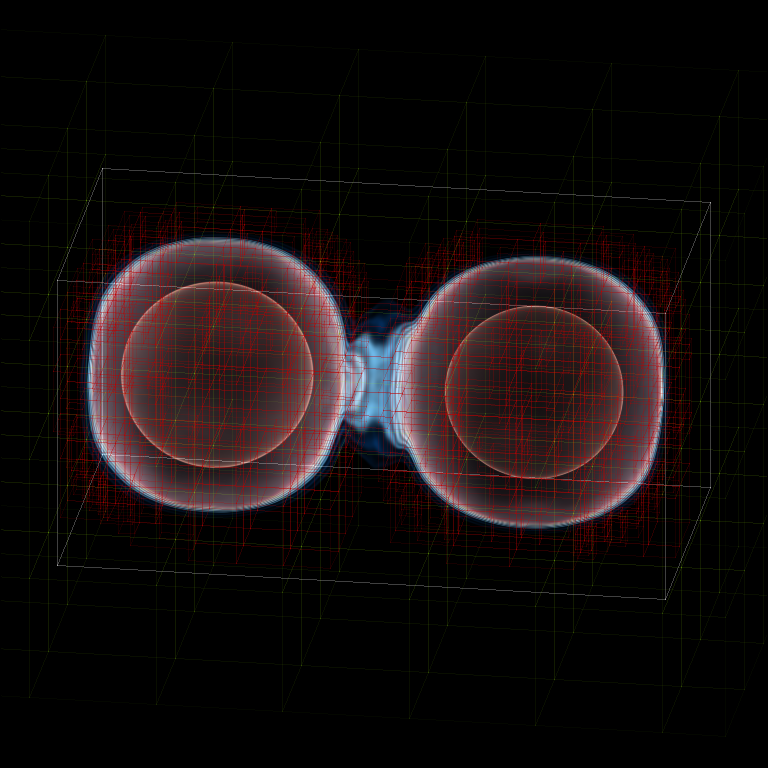
\includegraphics[width=3.5in]{volume}
\caption{Volume rendering}
\end{figure}
%%%%%%%%%%%%%%%%%%%%%%%%%%%%%%%%%


{\it\#------------------------}

{\it\# Isocontour Rendering}
{\setlength{\parskip}{0pt}

{\it\# Here we extract isocontours using some extra modules and plot them using matplotlib.}

from mpl\_toolkits.mplot3d import Axes3D
}

from mpl\_toolkits.mplot3d.art3d import Poly3DCollection

import matplotlib.pyplot as plt

from yt.mods import *

pf = load(`plt00020')

field = `pressure'

field\_weight = `magvel'

contour\_value = 2.83e13

domain = pf.all\_data()

{\it\# This object identifies isocontours at a given value for a given field. It returns}
{\setlength{\parskip}{0pt}

{\it\# the vertices of the triangles in that isocontour. It requires a data source, which}

{\it\# can be an object---but here we just give it all of our data. Here we find a pressure}

{\it\# isocontour and color it the magnitude of velocity over the same contour.}

surface = pf.surface(domain, field, contour\_value)
}

colors = apply\_colormap(np.log10(surface[field\_weight]), cmap\_name=`RdBu')

fig = plt.figure()

ax = fig.gca(projection=`3d')

p3dc = Poly3DCollection(surface.triangles, linewidth=0.0)

p3dc.set\_facecolors(colors[0,:,:]/255.)

ax.add\_collection(p3dc)

{\it\# By setting the scaling on the plot to be the same in all directions (using the x scale),}
{\setlength{\parskip}{0pt}

{\it\# we ensure that no warping or stretching of the data occurs.}

ax.auto\_scale\_xyz(surface.vertices[0,:], surface.vertices[0,:],
}

{\setlength{\parindent}{87pt}surface.vertices[0,:])}

ax.set\_aspect(1.0)

plt.savefig(`pres\_magvel\_isocontours.png')
%%%%%%%%%%%%%%%%%%%%%%%%%%%%%%%%%
\begin{figure}[h]
\centering
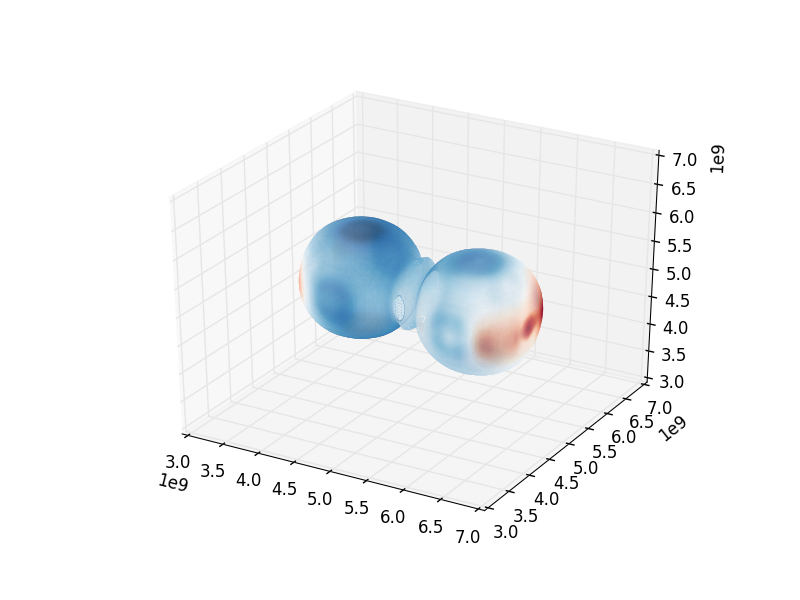
\includegraphics[width=4in]{isocontours}
\caption{Pressure isocontour rendering colored with velocity magnitude}
\end{figure}
%%%%%%%%%%%%%%%%%%%%%%%%%%%%%%%%%

{\it\#------------------------}

{\it\#1-D and 2-D Profiles}
{\setlength{\parskip}{0pt}

{\it\# Line plots and phase plots can be useful for analyzing data in detail.}

from yt.mods import *
}

pf = load(`plt00020')

pf.index

{\it\# Just like with the pressure\_contours script, we can set the units for fields that}
{\setlength{\parskip}{0pt}

{\it\# have none.}

pf.field\_info[`magvel'].\_units = r`\textbackslash rm\{cm\}/\textbackslash rm\{s\}'
}

pf.field\_info[`kineng'].\_units = r`\textbackslash rm\{ergs\}'

{\it\# We can create new fields from existing ones. \yt assumes all units are in cgs, and}
{\setlength{\parskip}{0pt}

{\it\# does not do any unit conversions on its own (but we can make it). Creating new fields}

{\it\#  requires us to define a function that acts on our data and returns the new data,}

{\it\# then call add\_field while supplying the field name, the function the data comes from,}

{\it\# and the units. Here, we create new fields simply to rename our data to make the plot}

{\it\# look prettier.}

def \_newT(field, data):
}

{\setlength{\parindent}{18.5pt}return data[`t']}

add\_field(`X', function=\_newT, units=r`\textbackslash rm\{domain\}\,\textbackslash rm\{fraction\}')

def \_newDen(field, data):

{\setlength{\parindent}{18.5pt}return data[`density']}

add\_field(`Density', function=\_newDen, units=r`\textbackslash rm\{g\}/\textbackslash rm\{cm\}\^{}\{3\}')

{\it\# PlotCollections are one of the most commonly used tools in \yt, alongside SlicePlots and}
{\setlength{\parskip}{0pt}

{\it\# ProjectionPlots. They are useful when we want to create multiple plots from the same}

{\it\# parameter file, linked by common characteristics such as the colormap, its bounds, and}

{\it\# the image width. It is easy to create 1-D line plots and 2-D phase plots through a}

{\it\# PlotCollection, but we can also create thin projections and so on. When we create a}

{\it\# PlotCollection, it is empty, and only requires the parameter file and the 'center' that}

{\it\# will be supplied to plots like slices and sphere plots.}

pc = PlotCollection(pf, `c')
}

{\it\# Now we add a ray---a sample of our data field along a line between two points we define}
{\setlength{\parskip}{0pt}

{\it\# in the function call.}

ray = pc.add\_ray([0.0, 5.0e9, 5.0e9],[1.e10, 5.0e9, 5.0e9], `magvel')
}

{\it\# This is where our derived fields come in handy. Our ray is drawn along the x-axis}
{\setlength{\parskip}{0pt}

{\it\# through the center of the domain, but by default the fraction of the ray we have gone}

{\it\# along is called `t.' We now have the same data in another field we called `X,' whose}

{\it\# name makes more sense, so we'll reassign the ray's first field to be that. If we wanted,}

(\it\# we could also reassign names to `magvel' and `kineng.'

ray.fields = [`X', `magvel']
}

{\it\# Next, we'll create a phase plot. The function requires a data source, and we can't}
{\setlength{\parskip}{0pt}

{\it\# just hand it our parameter file, but as a substitute we can quickly create an object}

{\it\# that spans our entire domain (or use the method in the isocontour example). The}

{\it\#  specifications of the region (a box) are the center, left bound, and right bound.}

region = pf.region([5.0e9, 5.0e9, 5.0e9], [0.0, 0.0, 0.0],
}

{\setlength{\parindent}{100pt}[1.0e10, 1.0e10, 1.0e10])}

{\it\# The phase object accepts a data source, fields, a weight, a number of bins along both}
{\setlength{\parskip}{0pt}

{\it\# axes, and several other things, including its own colormap, logarithm options,}

{\it\# normalization options, and an accumulation option. The first field is binned onto}

{\it\# the x-axis, the second field is binned onto the y-axis, and the third field is}

{\it\# binned with the colormap onto the other two. Subsequent fields go into an underlying}

{\it\# profile and do not appear on the image.}

phase = pc.add\_phase\_object(region, [`Density', `magvel',`kineng'], weight=None,
}

{\setlength{\parindent}{143pt}x\_bins=288, y\_bins=288)}

pc.save(`profile')
%%%%%%%%%%%%%%%%%%%%%%%%%%%%%%%%%
\begin{figure}[h]
  \centering
  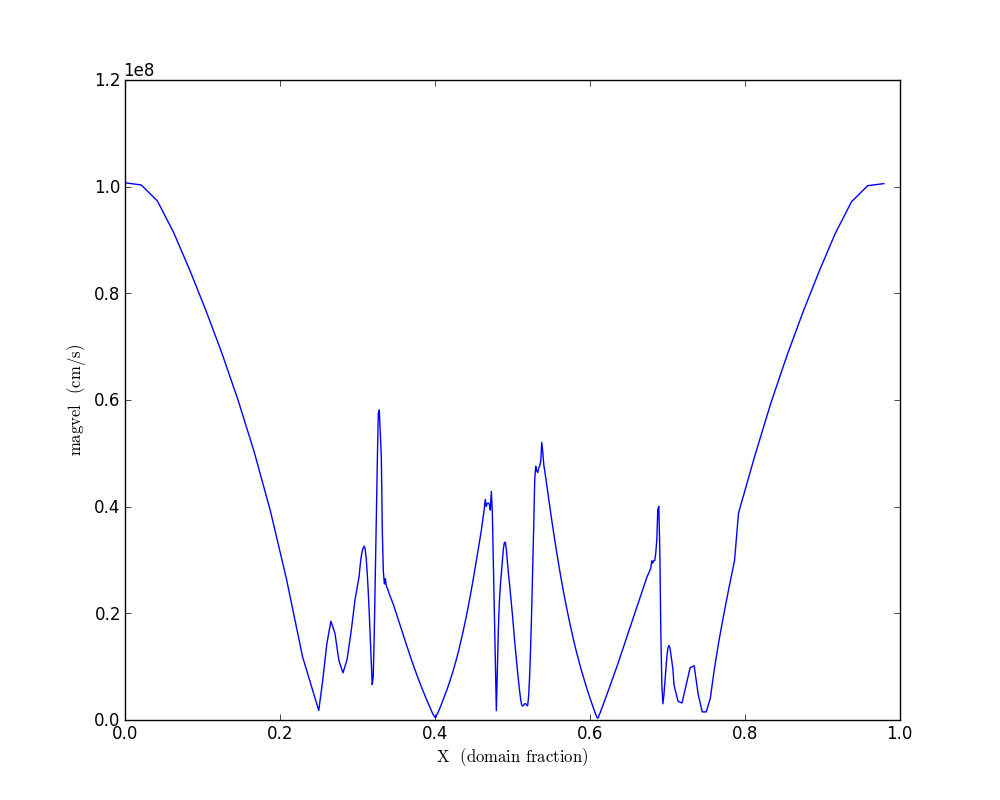
\includegraphics[width=4.0in]{LineQueryPlot_0_t_magvel}
  \caption{1-D velocity magnitude profile}
  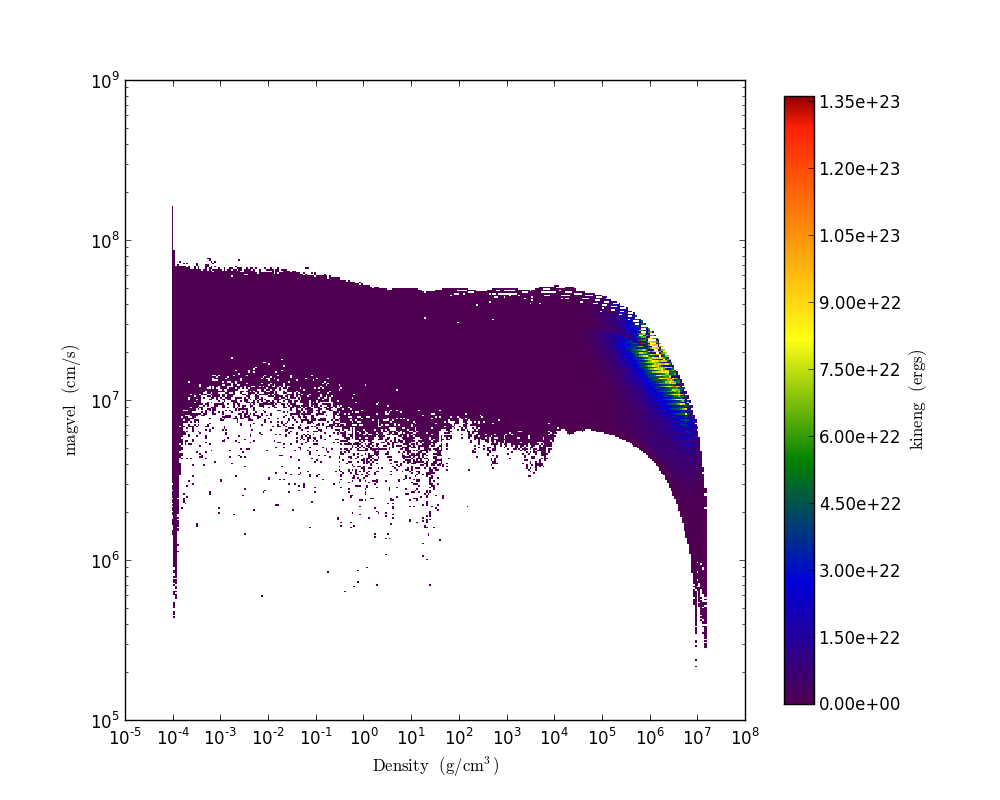
\includegraphics[width=4.0in]{Profile2D_1_Density_magvel_kineng}
  \caption{Density/velocity magnitude/kinetic energy phase plot}
\end{figure}
\quad
%%%%%%%%%%%%%%%%%%%%%%%%%%%%%%%%%

{\it\#------------------------}

{\it\#Off-Axis Projection}
{\setlength{\parskip}{0pt}

{\it\# If we don't want to take a projection (this can be done for a slice as well) along}

{\it\# one of the coordinate axes, we can take one from any direction using an}

{\it\# OffAxisProjectionPlot. To accomplish the task of setting the view up, the plot}

{\it\# requires some of the same parameters as the camera object: a normal vector, center,}

{\it\# width, and field, and optionally we can set no\_ghost (default is False). The normal}

{\it\# vector is automatically normalized as in the case of the camera. The plot also}

{\it\# requires a depth---that is, how much data we want to sample along the line of sight,}

{\it\# centered around the center. In this case `c' is a shortcut for the domain center.}

pf = load(`plt00020')
}

field = `density'

L = [0.25, 0.9, 0.40]

plot = OffAxisProjectionPlot(pf, L, field, center=`c',

{\setlength{\parindent}{146pt}width=(5.0e9, 4.0e9), depth=3.0e9)}

{\it\# Here we customize our newly created plot, dictating the font, colormap, and title.}
{\setlength{\parskip}{0pt}

{\it\# Logarithmic data is used by default for this plot, so we turn it off.}

plot.set\_font(\{`family':`Bitstream Vera Sans', `style':`italic',
}

{\setlength{\parindent}{63.5pt}`weight':`normal', `size':14, `color':`red'\})}

plot.set\_log(field, False)

plot.set\_cmap(field, `jet')

plot.annotate\_title(`Off-Axis Density Projection')

{\it\# The actual size of the image can also be set. Note that the units are in inches.}
{\setlength{\parskip}{0pt}

plot.set\_window\_size(8.0)
}

plot.save(`off\_axis\_density')
%%%%%%%%%%%%%%%%%%%%%%%%%%%%%%%%%
\begin{figure}[h]
  \centering
  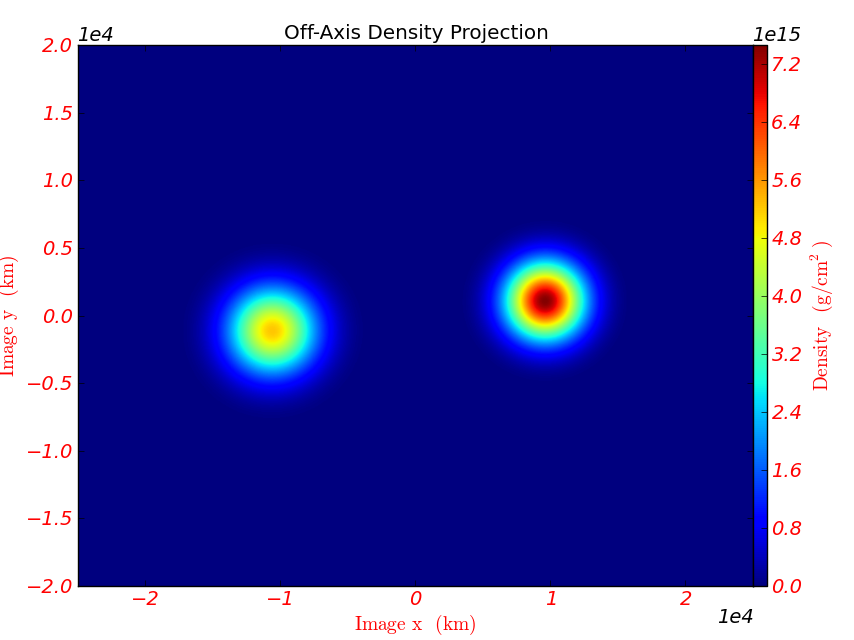
\includegraphics[width=4in]{OffAxisProjection_density}
  \caption{Off-axis density projection}
\end{figure}
%%%%%%%%%%%%%%%%%%%%%%%%%%%%%%%%%


\section{1D}

amrvis doesn't like 1-d plotfiles, and for those we use a 1-d plotting
capability installed by Mike Singer Castro/Util/plot1d.  If you want
to make xmgrace-compatible files, for example, add the following to
your inputs file:\\

{\bf xgraph.xmgrace\_file} = 1

{\bf xgraph.format} = xmg

{\bf xgraph.use\_xmgrace\_legend} = 1

{\bf xgraph.use\_xmgrace\_title} = 1

{\bf xgraph.graph} = xvel x\_velocity 100 -1\\ \\
This tells it to write a file called xvel\_0000.xmgr, for example, every 100 time steps, including all levels of data. (The last variable, -1, specifies the maximum level; if it is -1 then all levels are used.)

If you want to write more than one variable into a single file, then instead of
setting each variable on a separate line as in the xvel example above,
you can do the following: \\

\noindent {\bf xgraph.graph} = file\_name ALL 100 -1\\

\noindent If you specify ``ALL'' then \\

\noindent {\bf amr.plot\_vars} = \\

\noindent and \\

\noindent {\bf amr.derive\_plot\_vars} = \\

\noindent are used to control which variables are included.  The default for {\bf amr.plot\_vars}
is all of the state variables.  The default for {\bf amr.derive\_plot\_vars} is none of
the derived variables.  So if you include neither of these lines then the file 
file\_name.xmg will contain all of the state variables and none of the derived variables.

If you want all of the state variables plus entropy and pressure, for example, then set \\

{\bf amr.derive\_plot\_vars} = entropy pressure \\

{\bf xgraph.graph} = file\_name ALL 100 -1\\

If you just want density and pressure, for example, then set \\

{\bf amr.plot\_vars} =  density \\

{\bf amr.derive\_plot\_vars} = pressure \\

{\bf xgraph.graph} = file\_name ALL 100 -1\\ 

Feel free to read the routines in Castro/Util/plot1d.

